%!TEX TS-program = xelatex
\documentclass[12pt, a4paper, oneside]{article}

\usepackage{amsmath,amsfonts,amssymb,amsthm,mathtools}  % пакеты для математики

\usepackage[english, russian]{babel} % выбор языка для документа
\usepackage[utf8]{inputenc} % задание utf8 кодировки исходного tex файла
\usepackage[X2,T2A]{fontenc}        % кодировка

\usepackage{fontspec}         % пакет для подгрузки шрифтов
\setmainfont{Linux Libertine O}   % задаёт основной шрифт документа

\usepackage{unicode-math}     % пакет для установки математического шрифта
\setmathfont[math-style=upright]{Neo Euler} % шрифт для математики


%%%%%%%%%% Работа с картинками %%%%%%%%%
\usepackage{graphicx}                  % Для вставки рисунков
\usepackage{graphics}
\graphicspath{{images/}{pictures/}}    % можно указать папки с картинками
\usepackage{wrapfig}                   % Обтекание рисунков и таблиц текстом

%%%%%%%%%%%%%%%%%%%%%%%% Графики и рисование %%%%%%%%%%%%%%%%%%%%%%%%%%%%%%%%%
\usepackage{tikz, pgfplots}  % язык для рисования графики из latex'a

%%%%%%%%%% Гиперссылки %%%%%%%%%%
\usepackage{xcolor}              % разные цвета

\usepackage{hyperref}
\hypersetup{
	unicode=true,           % позволяет использовать юникодные символы
	colorlinks=true,       	% true - цветные ссылки, false - ссылки в рамках
	urlcolor=blue,          % цвет ссылки на url
	linkcolor=red,          % внутренние ссылки
	citecolor=green,        % на библиографию
	pdfnewwindow=true,      % при щелчке в pdf на ссылку откроется новый pdf
	breaklinks              % если ссылка не умещается в одну строку, разбивать ли ее на две части?
}


\usepackage{todonotes} % для вставки в документ заметок о том, что осталось сделать
% \todo{Здесь надо коэффициенты исправить}
% \missingfigure{Здесь будет Последний день Помпеи}
% \listoftodos --- печатает все поставленные \todo'шки

\usepackage[paper=a4paper, top=20mm, bottom=15mm,left=20mm,right=15mm]{geometry}
\usepackage{indentfirst}       % установка отступа в первом абзаце главы

\usepackage{setspace}
\setstretch{1.15}  % Межстрочный интервал
\setlength{\parskip}{4mm}   % Расстояние между абзацами
% Разные длины в латехе https://en.wikibooks.org/wiki/LaTeX/Lengths


\usepackage{xcolor} % Enabling mixing colors and color's call by 'svgnames'

\definecolor{MyColor1}{rgb}{0.2,0.4,0.6} %mix personal color
\newcommand{\textb}{\color{Black} \usefont{OT1}{lmss}{m}{n}}
\newcommand{\blue}{\color{MyColor1} \usefont{OT1}{lmss}{m}{n}}
\newcommand{\blueb}{\color{MyColor1} \usefont{OT1}{lmss}{b}{n}}
\newcommand{\red}{\color{LightCoral} \usefont{OT1}{lmss}{m}{n}}
\newcommand{\green}{\color{Turquoise} \usefont{OT1}{lmss}{m}{n}}

\usepackage{titlesec}
\usepackage{sectsty}
%%%%%%%%%%%%%%%%%%%%%%%%
%set section/subsections HEADINGS font and color
\sectionfont{\color{MyColor1}}  % sets colour of sections
\subsectionfont{\color{MyColor1}}  % sets colour of sections

%set section enumerator to arabic number (see footnotes markings alternatives)
\renewcommand\thesection{\arabic{section}.} %define sections numbering
\renewcommand\thesubsection{\thesection\arabic{subsection}} %subsec.num.

%define new section style
\newcommand{\mysection}{
	\titleformat{\section} [runin] {\usefont{OT1}{lmss}{b}{n}\color{MyColor1}} 
	{\thesection} {3pt} {} } 


%	CAPTIONS
\usepackage{caption}
\usepackage{subcaption}
%%%%%%%%%%%%%%%%%%%%%%%%
\captionsetup[figure]{labelfont={color=Turquoise}}

\pagestyle{empty}


%%%%%%%%%% Свои команды %%%%%%%%%%
\usepackage{etoolbox}    % логические операторы для своих макросов

% Все свои команды лучше всего определять не по ходу текста, как это сделано в этом документе, а в преамбуле!

% Одно из применений - уничтожение какого-то куска текста!
\newbool{answers}
%\booltrue{answers}
\boolfalse{answers}

\begin{document}

\section*{Семинар 2-3:  сегментация клиентов и кластеризация}

\subsection*{Задача 1 }

\begin{enumerate}

\item У нас есть точки $A(1,1)$, $B(2,2)$, $C(3,0)$. Нарисуйте их на плоскости и посчитайте между ними расстояние Евклида, Манхеттенское и Чебышева: 

\[ \rho(A,B) = \sqrt{(x_B - x_A)^2 + (y_B - y_A)^2} \]

\[\rho(A,B) = |x_B - x_A| + |y_B - y_A|  \]

\[ \rho(A,B) = \max(|x_B - x_A|, |y_B - y_A|) \]


\item Какое расстояние будете использовать для того, чтобы посчитать расстояние между точками А и Б для случаев ниже? Почему? 

\begin{minipage}[t]{0.45\textwidth}
	\includegraphics[scale=0.12]{metr_1.png}
\end{minipage}
\hfill
\begin{minipage}[t]{0.45\textwidth}
	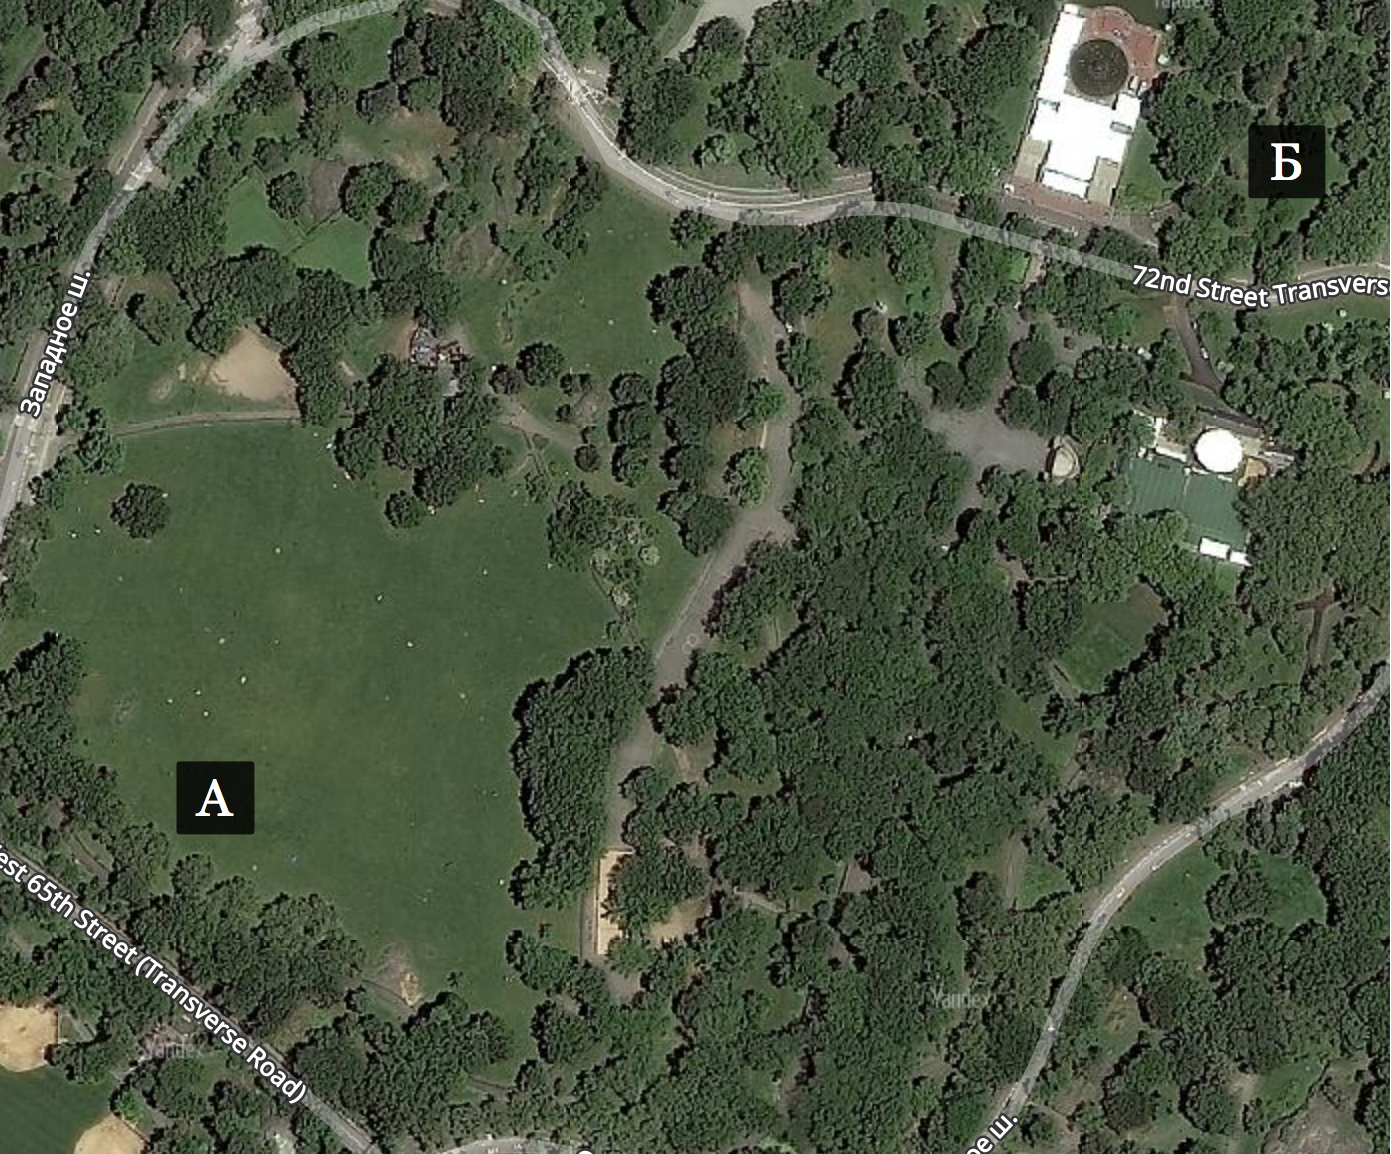
\includegraphics[scale=0.12]{metr_2.png}
\end{minipage}

\item Какое расстояние вы бы использовали для измерения похожести текстов или генома?

\begin{center}
	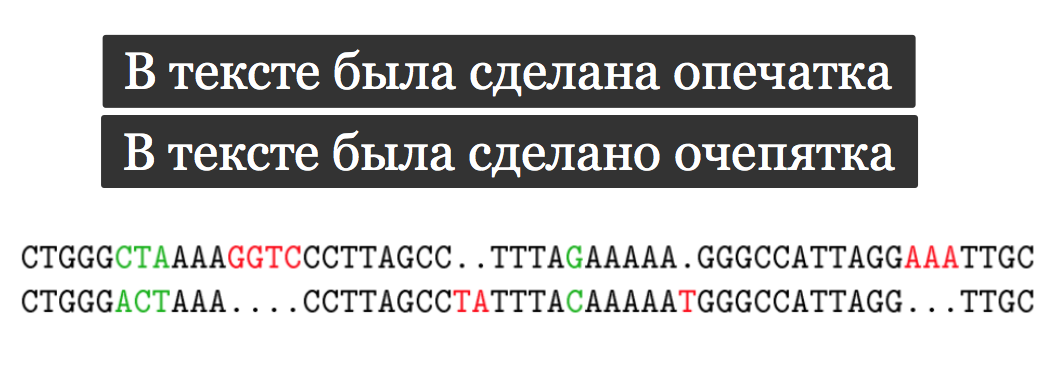
\includegraphics[scale=0.3]{metr_3.png}
\end{center}


\end{enumerate}


\subsection*{Задача 2}

Жокей Святополк решил открыть несколько новых ларьков с шаурмой\footnote{По мотивам \url{https://vas3k.ru/blog/machine_learning/}}. Перед открытием он подумал о потенциальных покупателях и выяснил, где на районе находятся общежития.  На картинках ниже они отмечены синими точками.  Святополк понимает, что все общежития, расположенные в районе, можно сегментировать по их географическому положению и, исходя из этого, расположить палатки с шаурмой. Сделать  это ему хотелось бы с помощью алгоритма $K-means$:

\begin{enumerate}
	\item Ставим ларьки с шаурмой в случайных местах;
	\item Смотрим в какой кому ближе идти;
	\item Двигаем ларьки ближе к центрам их популярности;
	\item Снова смотрим и двигаем;
	\item Повторяем так много раз, пока алгоритм не сойдётся и движение не прекратится.
\end{enumerate}

\begin{minipage}[t]{0.45\textwidth}
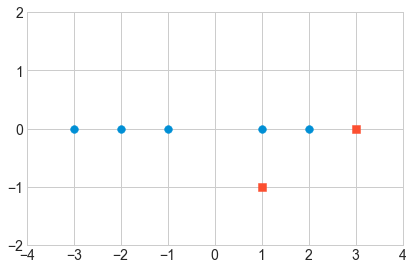
\includegraphics[scale=0.5]{knn1.png}
\end{minipage}
\hfill
\begin{minipage}[t]{0.45\textwidth}
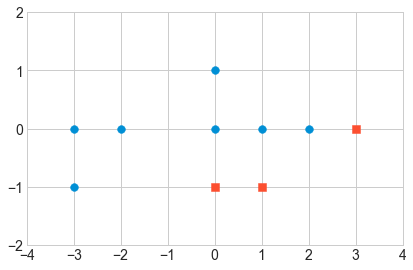
\includegraphics[scale=0.5]{knn2.png}
\end{minipage}

Красными точками отмечены стартовые точки для палаток. В первом районе Святополк ставит две палатки, во втором районе три палатки.  Помогите Святополку с сегментацией! Сколько итераций понадобилось сделать до полной сходимости алгоритма? Сколько объектов вошли в каждый из кластеров?  

\begin{enumerate}
	\item[а)] Используйте для кластеризации Евклидово расстояние.
	\item[б)] Используйте для кластеризации Манхеттенское расстояние.
	\item[в)] В этой задачке мы сами предложили вам для кластеризации начальные точки (красные квадраты). На практике начальное приближение центроидов обычно генерирует компьютер.  Изменится ли разбиение на кластеры, если изменить стартовые точки?
\end{enumerate}


\subsection*{Задача 3 }

Начальник Аристарх был в командировке. Там он услышал про иерархическую агломеративную кластеризацию. По приезду, находясь в состоянии восторга, он записал в свой блокнот следующие четыре наблюдения:

\begin{center}
\begin{tabular}{c|c}
	\hline
	$x$ & $z$ \\
	\hline
	8 & 6   \\
	6 & 10 \\
	2 & 4   \\
	4 & 2   \\
\end{tabular}
\end{center}

После он отдал блокнот маркетологу Савелию. Аристарх хочет, чтобы Савелий провел агломеративную иерархическую кластеризацию.  На совещаний было решено использовать в качестве расстояния между объектами обычное Евклидово расстояние. Расстояние между кластерами решено определять по принципу дальнего соседа. Помогите Савелию с агломеративной иерархической кластеризацией. И не забудьте нарисовать дендрограмму. Начальники любят красивые картинки. 

\subsection*{Задача 4} 

Маркетолог с аналитическим складом ума Оля (она кстати говоря ещё и фрилансер) занимается заказом от туристической фирмы. Ей нужно сделать с помощью методов машинного обучения сегментацию клиентов. На этапе предобработки фичей Оля столкнулась с двумя проблемами: категориальной переменной $x$, в которой записаны курорты и текстовой переменной $z$, в которой дан отзыв о курорте:

\begin{center}
	\begin{tabular}{c|c|c}
		\hline
		$n$ & $x$ & $z$ \\
		\hline
		1 & Испания  & Нежился на пляже  \\
		2 & Крым  &  Копали яму на пляже\\
		3 & Дача  &  Копал картошку  \\
		4 & Крым  & Ел картошки и картошку \\
	\end{tabular}
\end{center}

\begin{enumerate} 
	\item  Что такое категориальная переменная? Почему её надо как-то предобрабатывать? 
	\item  Почему нельзя сделать замену Крым $=1$, Дача $=2$, Испания $=3$? Что такое OHE-кодирование? Как будет выглядеть наша табличка с переменными после OHE?
	\item  Почему нельзя сделать OHE для текстовой переменной?
	\item  Какие этапы предобработки тестов вы знаете? На самом деле вы их скорее всего не знаете и мы их сейчас обсудим. 
	\item Сделайте для корпуса текстов из задачки tf-idf. 
\end{enumerate}


\section*{Ещё задачи!}

\subsection*{Задача 5} 

Представьте себе, что вы шахматная фигура. Какое расстояние вы бы использовали, чтобы измерить насколько далёкий путь вам предстоит пройти по шахматной доске.  Придумайте метрику для каждой шахматной фигуры: ладья, слон, ферзь, король, слон, конь. Попытайтесь формализовать эту метрику в виде формулы. 

\textbf{Подсказка:}  попробуйте нарисовать шахматную доску на бумажке, поставить в какую-нибудь клетку фигуру, а после для каждой клетки выписать цифру: сколько до этой клетки идти фигуре.  Это поможет придумать для формулы общий вид. Клетку $a1$ в координатной сетке примите за $(0,0)$. 

% {если} {правда} {ложь}
\ifbool{answers}{
\textbf{Решение:}

Будем измерять расстояние в клетках, которые были пройдены фигурой. Другой подход --- измерять растояние в ходах. Это не очень коректно, так как в таком случае будет непонятно какая у фигур сокрость. 

Расстояние, которое преодалевает ладья будет измеряться с помощью манхеттенской метрики. 

\[ \rho(x,y) = |x_2 - x_1| + |y_2 - y_1| \]

Будем считать, что у клетки $a1$ координаты $(0,0)$. Тогда, если ладья хочет попаст из клетки $e6$ в клетку $b1$, то есть из $(4,5)$ в $(1,0)$, ей надо будет пройти $|1-4| + |0-5| = 3 + 5 = 8$ клеток. Обратите внимание, что все точки вокруг ладьи по мере отдаленмя от неё выстраиваются в концентрические ромбики с одинаковыми расстояниями. 

Для слона ситуация будет аналогичной. Для него используется манхеттенское расстояние, но доска для него повёрнута под углом $45$ градусов. 

\begin{minipage}[t]{0.45\textwidth}
	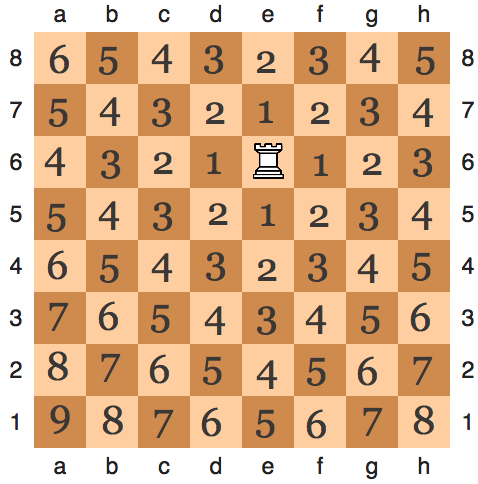
\includegraphics[scale=0.5]{ladia.png}
\end{minipage}
\hfill
\begin{minipage}[t]{0.45\textwidth}
	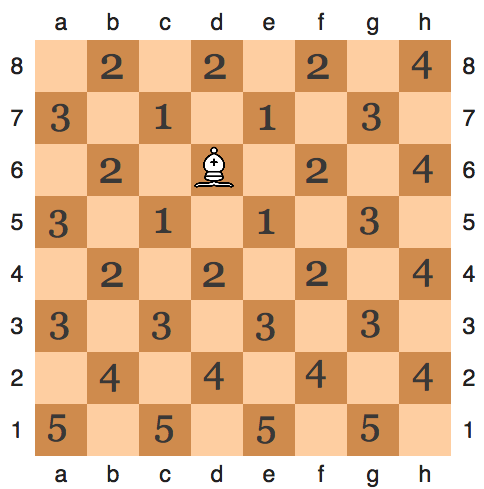
\includegraphics[scale=0.5]{slon.png}
\end{minipage}

Для короля и ферзя ситуация будет немного другой. Из-за того, что они могут ходить и по вертикали и по диагонали, их расстояние считается по формуле:

\[ \rho(x,y) = max( |x_2 - x_1|, |y_2 - y_1| ). \]

Тогда, если король хочет попасть из клетки $f6$ в клетку $b1$, то есть из $(5,5)$ в $(1,0)$, он должен пройти $\max(|1-5|, |0-5|) = \max(4, 5) = 5$. По сравнению с ладьёй, у короля есть приемущество. Для него клетки выстраиваются в концетрические квадраты. Диагонали для него в одношаговой доступности, когда для ладьи они в двухшаговой доступности. Расстояние, описанное выше называется расстоянием Чебышёва. 

\begin{minipage}[t]{0.45\textwidth}
	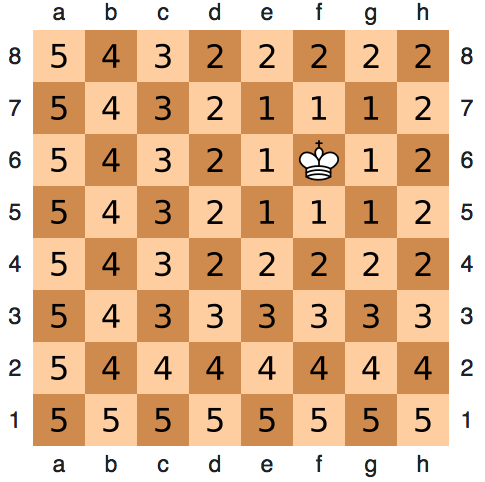
\includegraphics[scale=0.5]{king.png}
\end{minipage}
\hfill
\begin{minipage}[t]{0.45\textwidth}
	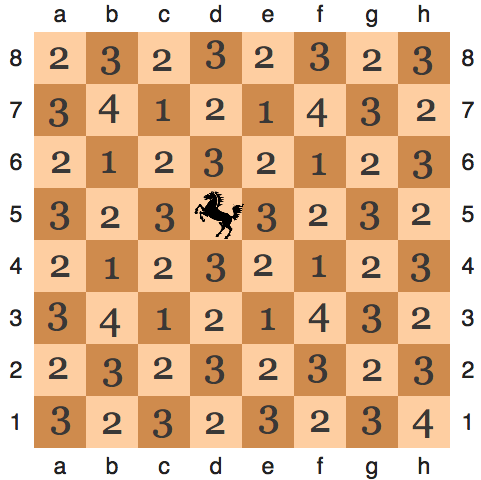
\includegraphics[scale=0.5]{koni.png}
\end{minipage}

Для коня ситуация оказывается самой загадочной. Из-за того, что он ходит буквой Г, расстояния, расчитываемые для него оказываются нелинейными. Их нельзя формализовать в виде простой формулы, но можно нарисовать. Концентрические линии для коня оказываются совсем чудными. Клетка, до которой идти $4$ хода с точки зреня привычных ддя нас расстояний, оказывается к коню ближе, чем клетка, до которой идти $3$ хода. 
}{ }


\subsection*{Задача 6} 

\begin{center}
	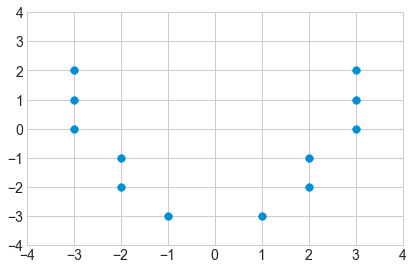
\includegraphics[scale=0.6]{knn_3.png}
\end{center}

\begin{enumerate}
	\item Примените метод $K$-means с $K=2$, $K=3$, $K=4$ и $K=5$. Начальные точки каждый раз выбирайте случайно.  Спишитесь с другими людьми и выясните какие точки они выбрали для инициализации. Для каких $K$ у вас получились одинаковые результаты? Почему?  
	
	\item Примените метод агломеративной иерархической кластеризации. Нарисуйте дендрограмму. Руководствуясь дендрограммой выберете оптимальное количество кластеров. Обоснуйте свой выбор.
	
	\item Правда ли, что для всех рассмотренных $K$ оба метода разбивают выборку на одинаковые кластеры?  Всегда ли так происходит? Докажите это или приведите контр-пример. 
	
	\item В первом пункте вы попробовали провести кластеризацию для разных $K$. Какое из $K$ является оптимальным? Для того, чтобы определить это используйте сумму квадратов расстояний от точек до центров кластеров. 
	
	\item Какое $K$ будет оптимальным, если вместо суммы квадратов расстояний от точек до центров кластеров использовать коэффициент силуэта? 		
\end{enumerate}


\subsection*{Задача 7} 

Обозначьте расположение центроидов и границ кластеров после применения метода K-means c $K=2$ на следущих данных: 

\begin{minipage}[t]{0.66\textwidth}
	\begin{center}
		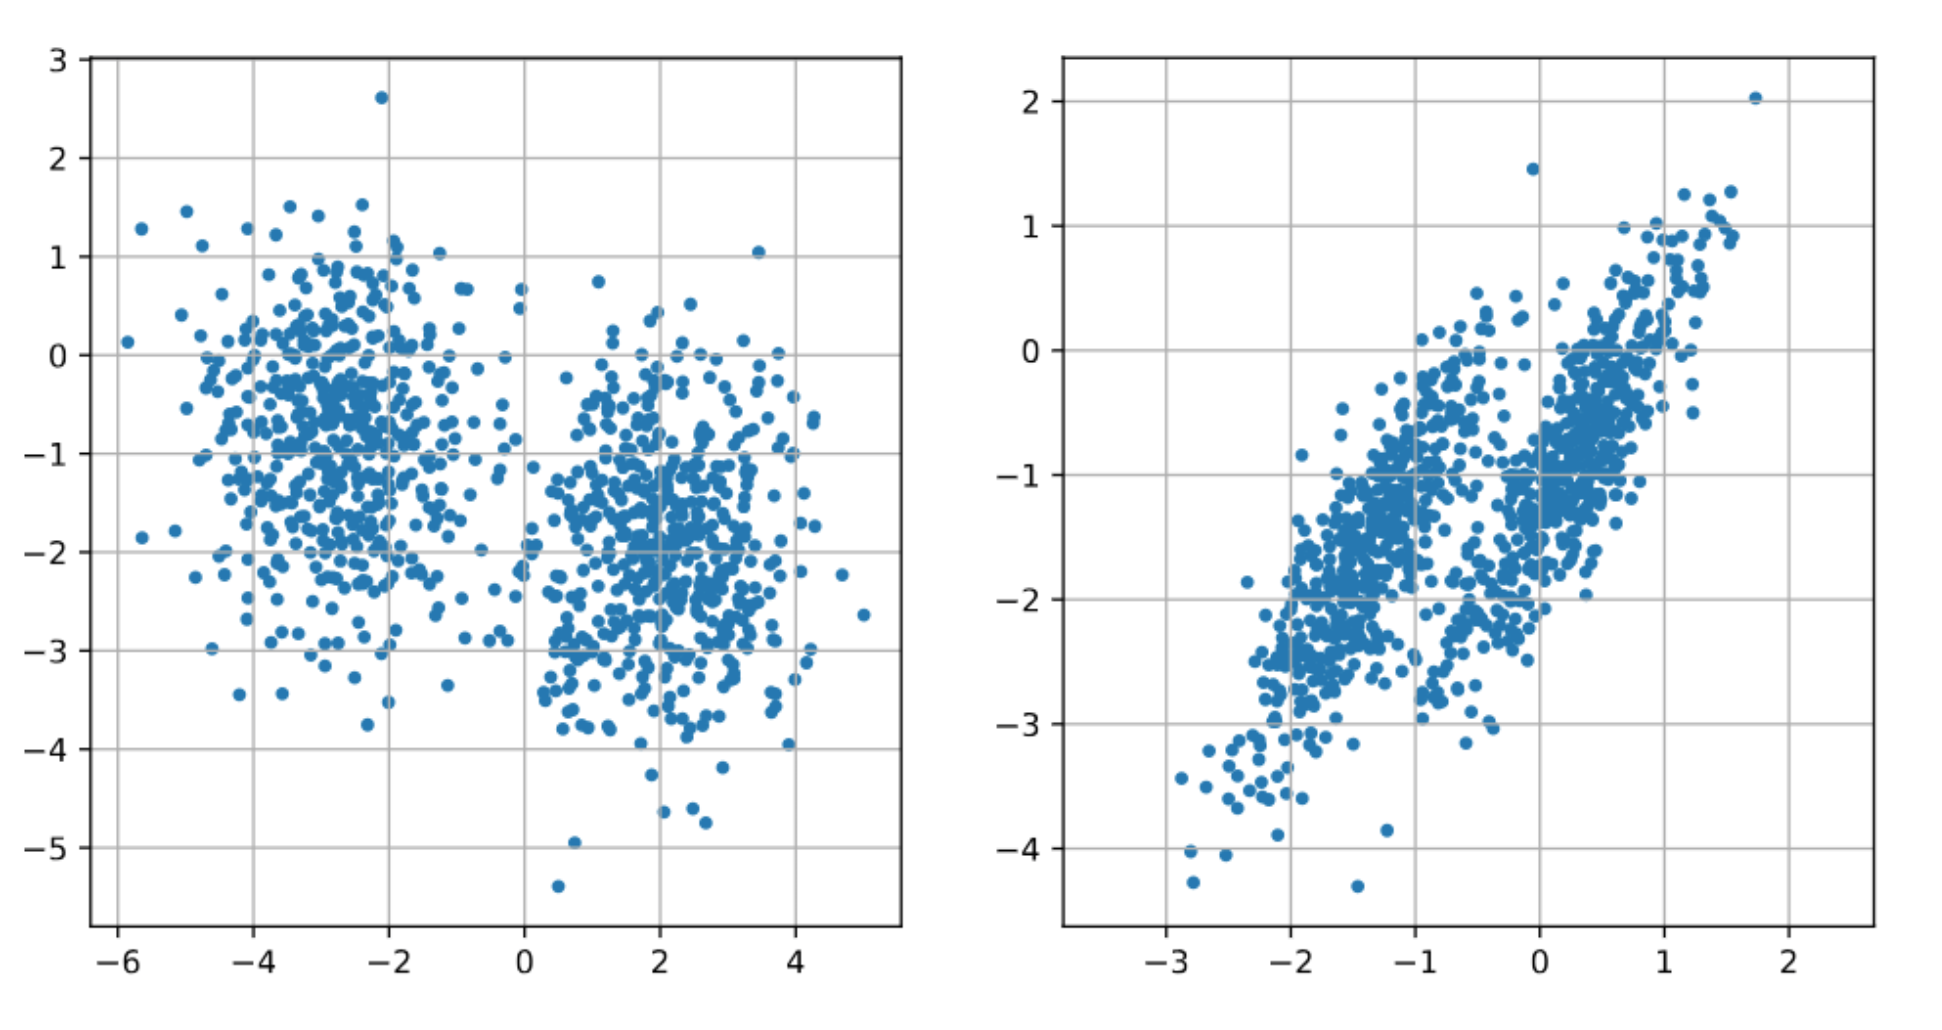
\includegraphics[scale=0.15]{clouds.png}
	\end{center}
\end{minipage}
\begin{minipage}[t]{0.33\textwidth}
	\begin{center}
		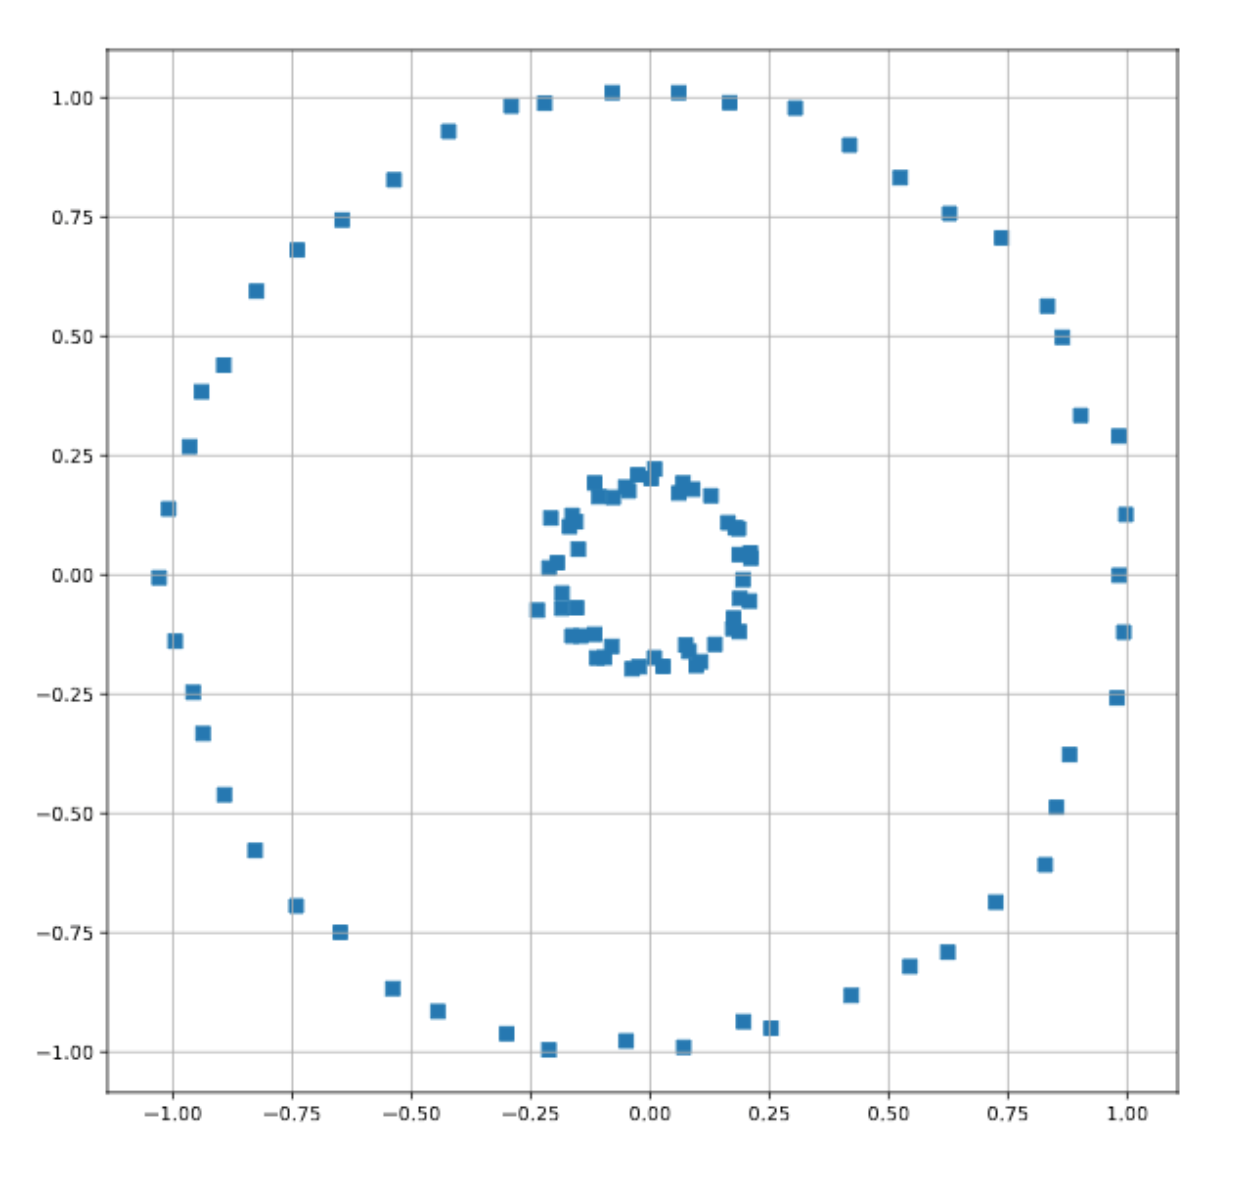
\includegraphics[scale=0.13]{circles.png}
	\end{center}
\end{minipage}

Если вы подумали, что это изи-задание и на третьей картинке сходу взяли в один кластер внутреннюю окружность, а во второй внешнюю - вы балбес. Это неправильно. Идите и подумайте ещё.
\end{document}
